\chapter{Mt. Gagazet}
\begin{enumerate}
    \item Walk up, \cs[3:40], walk up, \sd
\end{enumerate}
\begin{battle}{Biran and Yenke}
    \begin{itemize}
        \kimahrif Steal from Biran
        \enemyf Biran Bulldoze
        \kimahrif Gem Yenke
        \kimahrif Gem Biran
    \end{itemize}
    Pay attention to your drops, they affect \yuna's sphere grid below.
\end{battle}
\begin{enumerate}[resume]
    \item The drop from the previous fight will give be one of the following:
    \begin{itemize}
        \item \textbf{4 Return Spheres}
        \item \textbf{2 Return Spheres and 2 Friend Spheres}
        \item \textbf{0 Return Spheres and 4 Friend Spheres}
    \end{itemize}
    \item These three branching paths will from now on be referred to by the number of \textbf{Return Spheres} that dropped.
    \item Do the \lulu\ Grid below first, then one of the three Grids depending on the drop from the previous fight.
\end{enumerate}
\begin{spheregrid}[Lulu]
    \begin{itemize}
        \luluf
        \begin{itemize}
            \item Move $\uparrow\uparrow$
            \item Level 2 Key Sphere
            \item Move $\downarrow x9$
            \item Level 3 Key Sphere
            \item Move $\searrow\searrow$
        \end{itemize}
        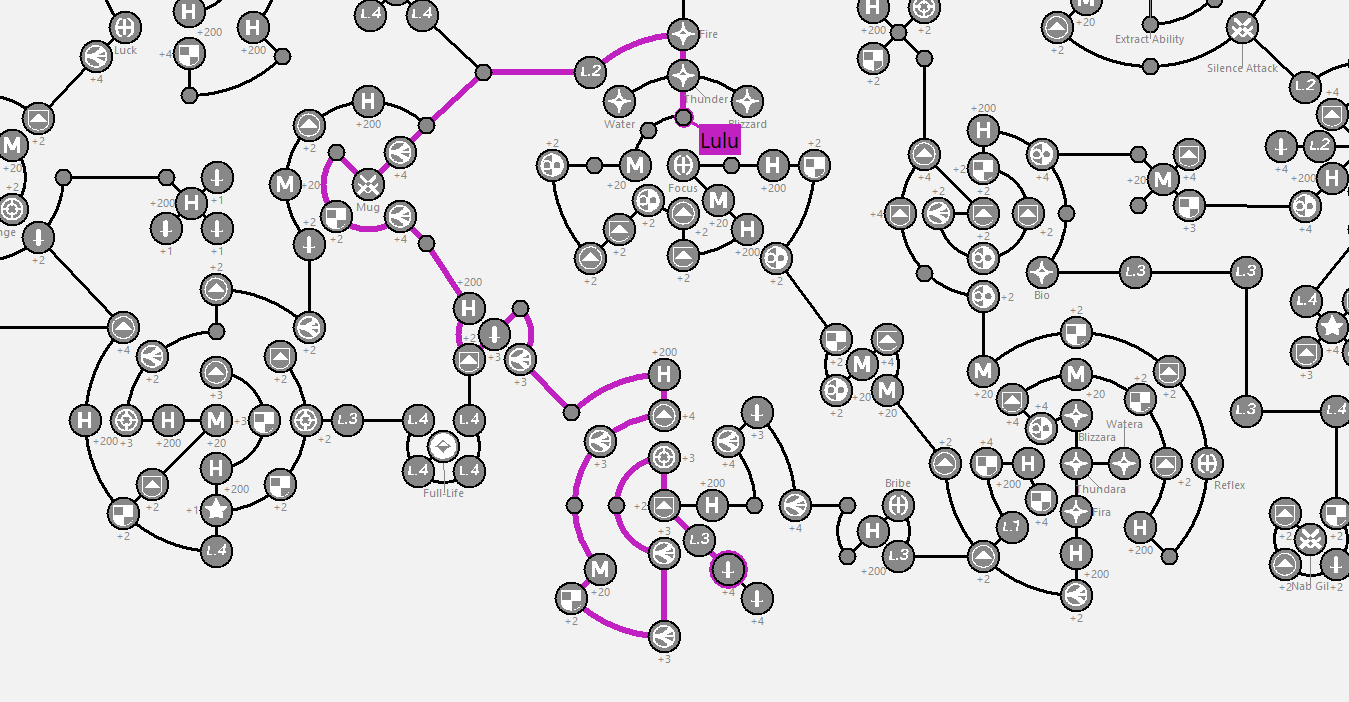
\includegraphics[width=.25\columnwidth]{graphics/lulu_grid}
    \end{itemize}
\end{spheregrid}
\begin{spheregrid}[\textbf{4 Return Spheres}]
    \begin{itemize}
        \blitzballdetermination[true]{%
            \yunaf Use Return Sphere to Str+4 Node
            \yunaf Move to the empty node $\leftarrow\downarrow$
            \yunaf Str+4, Agi+2
            \item 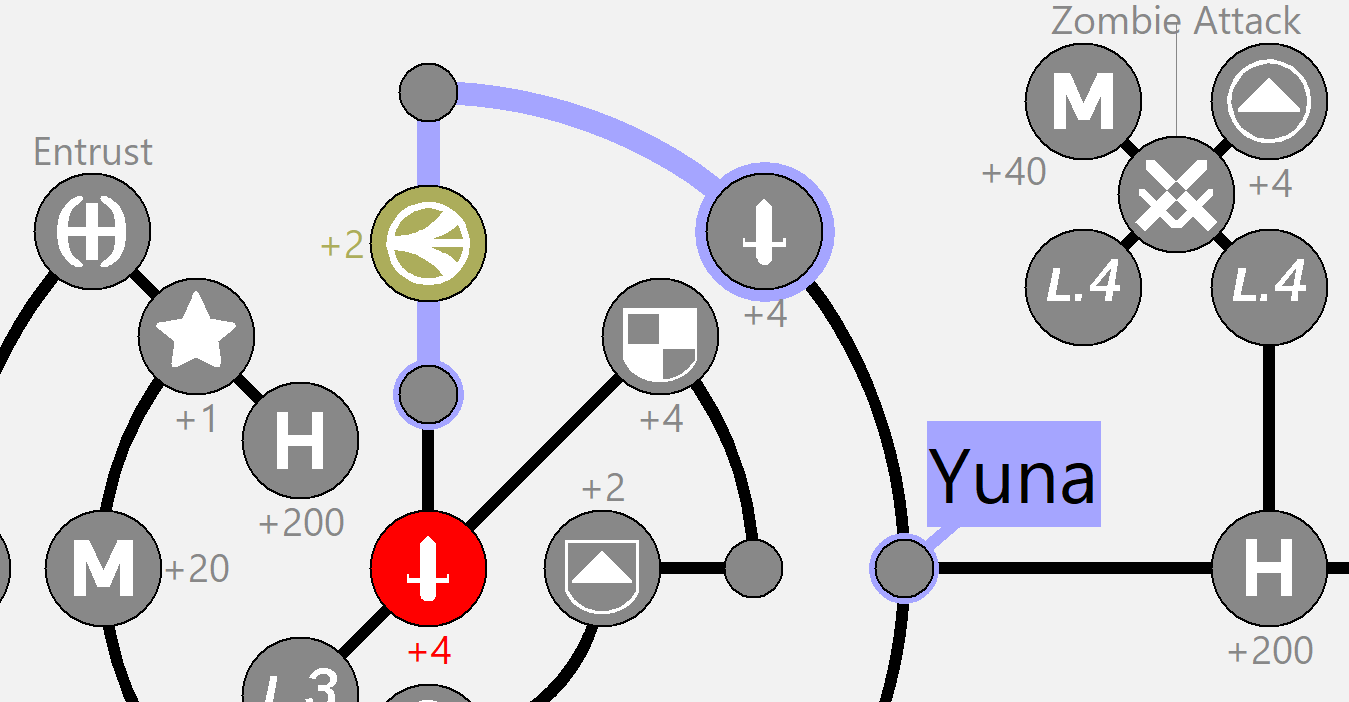
\includegraphics[width=.250\columnwidth]{graphics/4_returns_1}
        }{%
            \yunaf Use Return Sphere to Str+4 Node $\leftarrow$
            \yunaf Move to the empty node $\rightarrow\rightarrow\rightarrow$
            \yunaf Str+4, Def+3
            \item 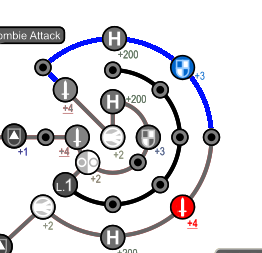
\includegraphics[width=.250\columnwidth]{graphics/loss_4_returns_1}
        }
        \tidusf Move to Armor Break $\rightarrow x3, \downarrow x5$
        \tidusf Armor Break
        \item 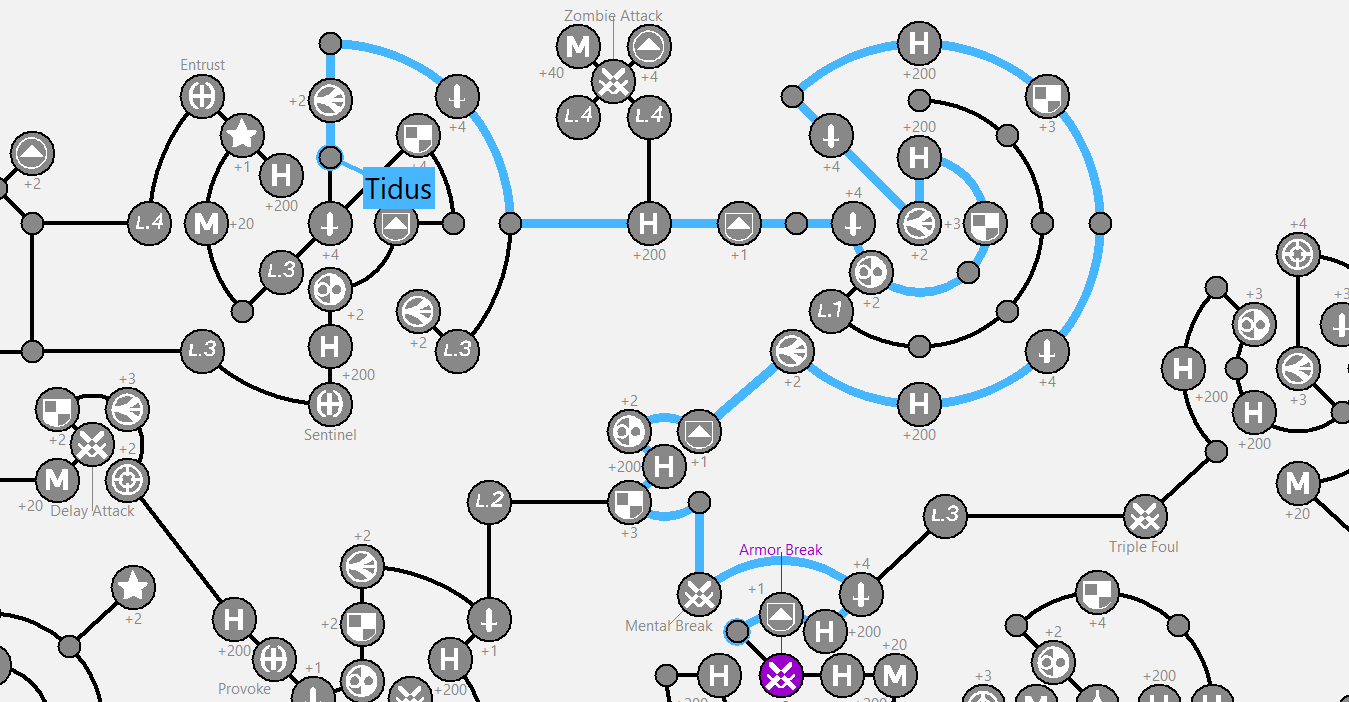
\includegraphics[width=.25\columnwidth]{graphics/Tidus armor break 4 returns}
    \end{itemize}
\end{spheregrid}
\begin{spheregrid}[\textbf{2 Return Spheres}]
    \begin{itemize}
        \blitzballdetermination[true]{%
            \yunaf Move to the empty node $\leftarrow$
            \yunaf Str+4, Agi+2
            \item 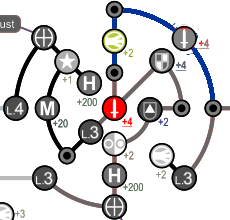
\includegraphics[width=.25\columnwidth]{graphics/2_and_2-1}
        }{%
            \yunaf Move to the empty node $\rightarrow\rightarrow$
            \yunaf Str+4, Def+3
            \item 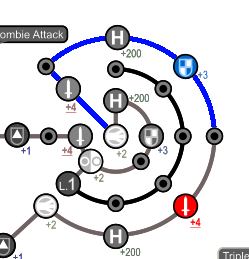
\includegraphics[width=.25\columnwidth]{graphics/loss_2_and_2-1}
        }
        \yunaf Friend Sphere to \lulu\ $\downarrow\downarrow$
        \yunaf Str+4, Str+4
        \luluf Move $\nearrow\uparrow\uparrow$
        \yunaf Friend Sphere to \lulu
        \yunaf Str+3, Agi+4, Agi+4
        \item 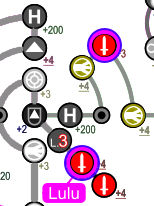
\includegraphics[width=.25\columnwidth]{graphics/2_and_2}
        \tidusf Return Sphere $\downarrow\searrow\searrow$ (or Hold $\searrow$) to Str+4 near Armor Break
        \tidusf Move $\nwarrow\leftarrow$ or $\leftarrow x3$
        \tidusf Armor Break
        \item 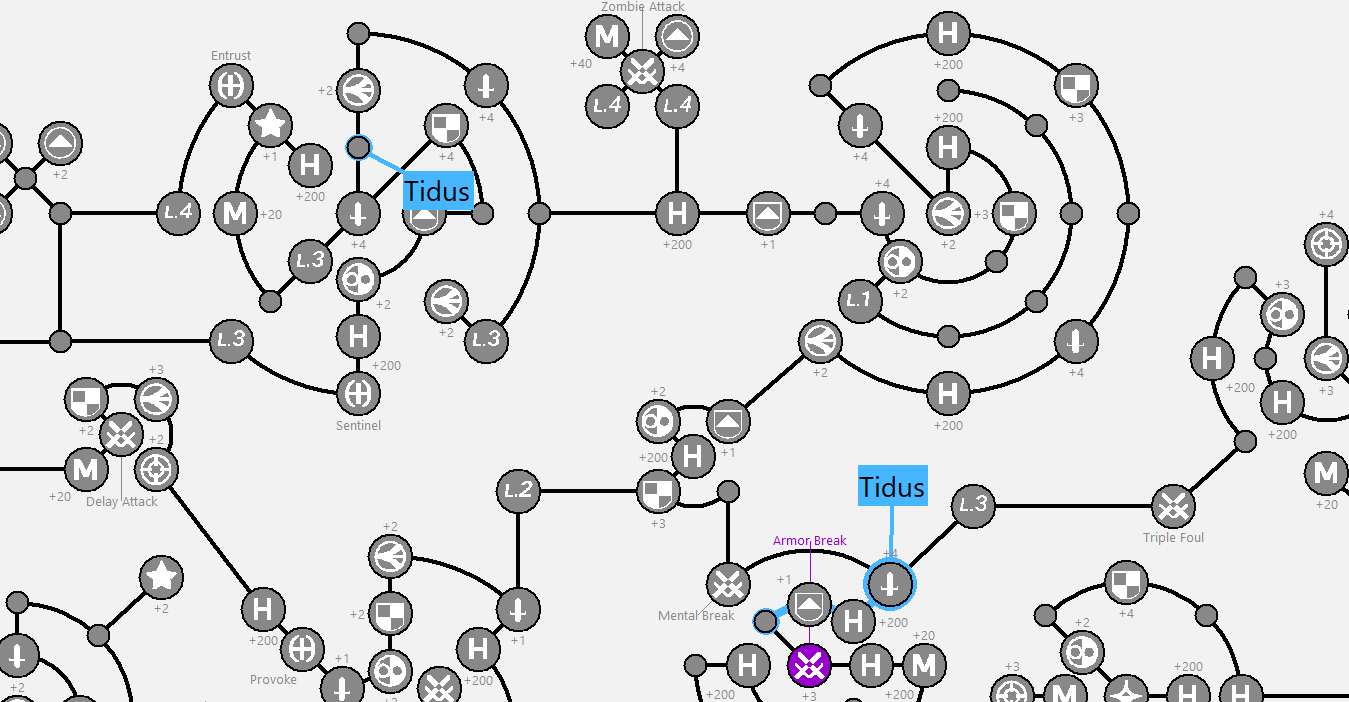
\includegraphics[width=.25\columnwidth]{graphics/Tidus armor break 2 returns}
    \end{itemize}
\end{spheregrid}
\begin{spheregrid}[\textbf{0 Return Spheres}]
    \begin{itemize}
        \blitzballdetermination[true]{%
            \tidusf Move to Str+4 by Mental Break $\rightarrow x3, \downarrow, \rightarrow x3$
            \item 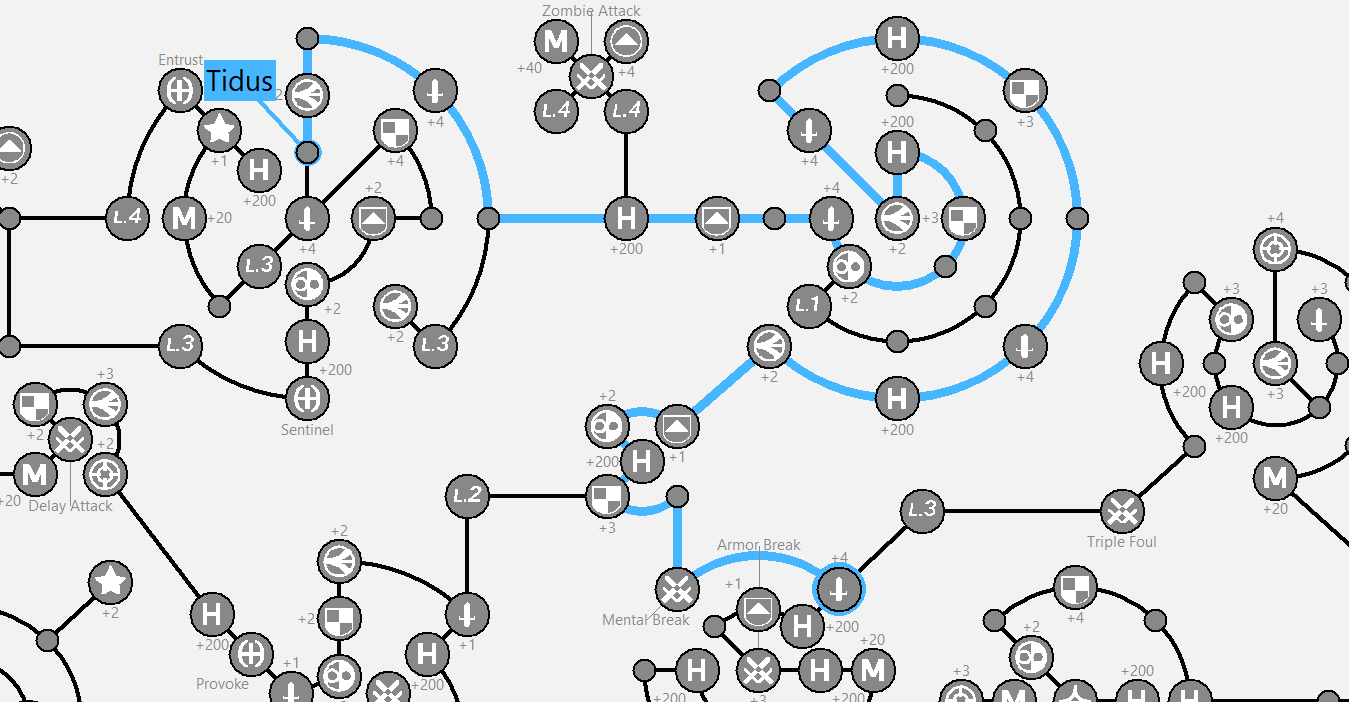
\includegraphics[width=.25\columnwidth]{graphics/0_returns_pt2}
            \yunaf Move to the empty node $\leftarrow$
            \yunaf Str+4, Agi+2
            \item 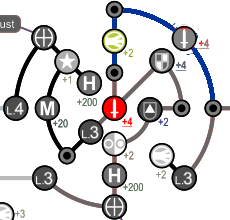
\includegraphics[width=.25\columnwidth]{graphics/2_and_2-1}
        }{%
            \tidusf Move to Armor Break $\rightarrow x3, \downarrow x6$
            \tidusf Armor Break
            \tidusf Move to HP $\rightarrow\rightarrow\downarrow$
            \yunaf Move to the empty node $\rightarrow\rightarrow$
            \yunaf Str+4, Def+3
            \item 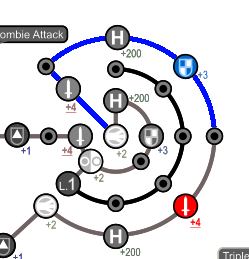
\includegraphics[width=.25\columnwidth]{graphics/loss_2_and_2-1}
        }
        \yunaf Friend Sphere to \tidus
        \yunaf Str+4
        \item Friend Sphere to Lulu twice like described \textbf{in the 2 Return Sphere Menu}
        \kimahrif Move $\swarrow x2$
        \yunaf Friend to \kimahri\ $\downarrow$
        \yunaf Agi+4
        \item 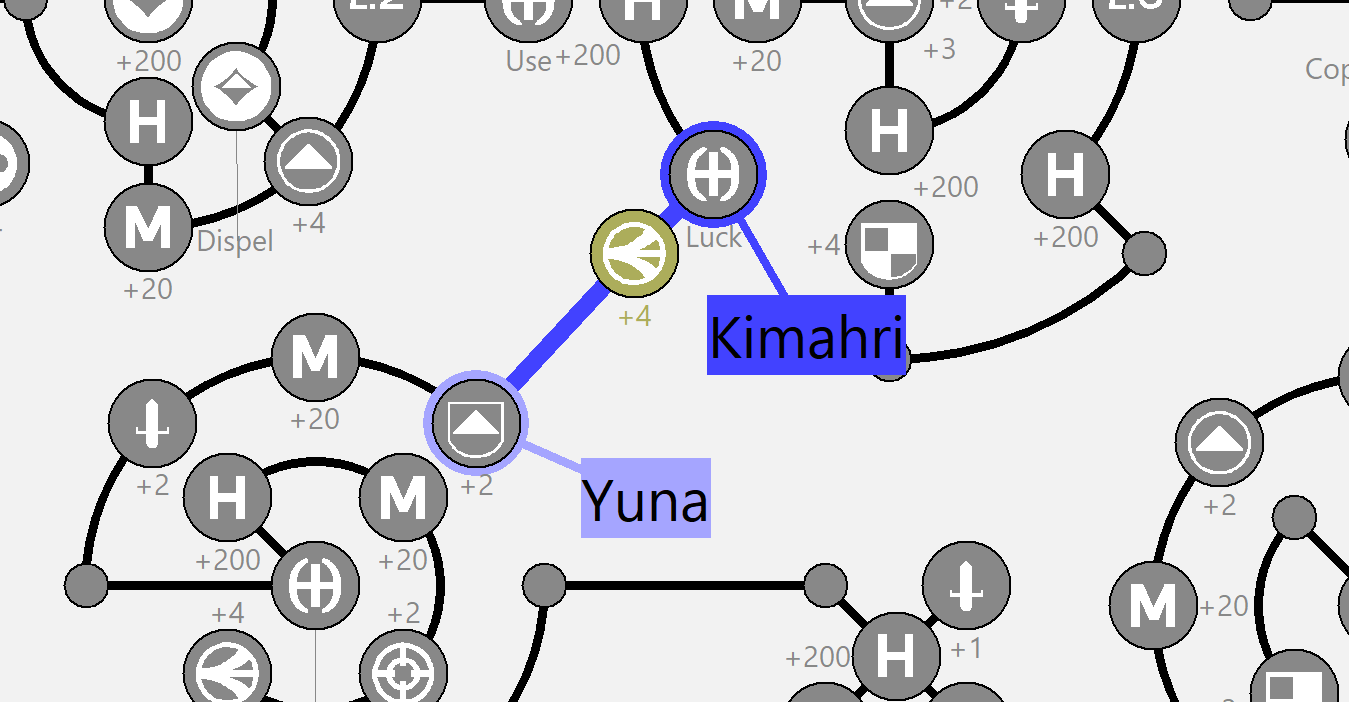
\includegraphics[width=.25\columnwidth]{graphics/post_BY_0_returns}
        \blitzballdetermination[true]{%
            \tidusf Move $\nwarrow\leftarrow$ or $\leftarrow x3$
            \tidusf Armor Break
            \item 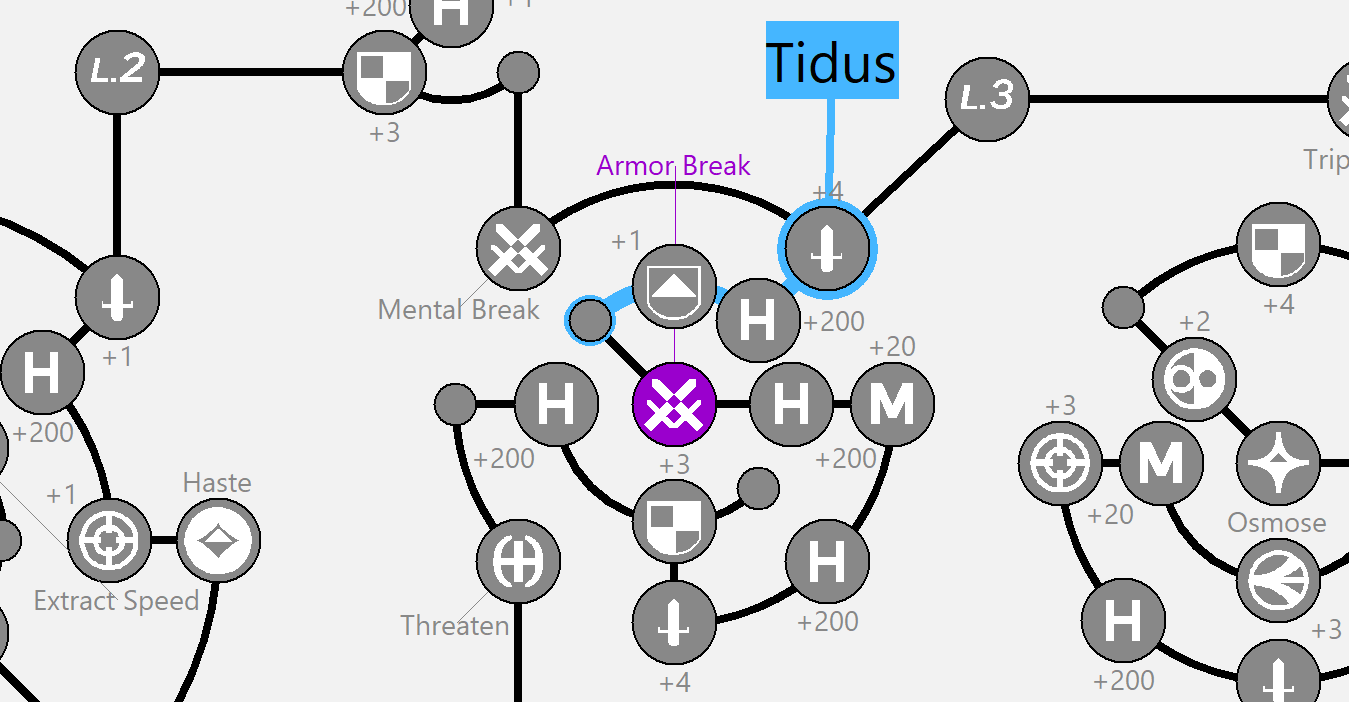
\includegraphics[width=.25\columnwidth]{graphics/Tidus armor break 0 returns}
        }{}
    \end{itemize}
\end{spheregrid}
\begin{enumerate}[resume]
    \item \textit{If you got \textbf{4 Return Spheres}:}
    \begin{itemize}
        \item Customize:
        \begin{itemize}
            \auronf Shimmering Blade $\rightarrow$ First Strike
            \yunaf Staff $\rightarrow$ First Strike
        \end{itemize}
    \end{itemize}
    \item \textit{If you got \textbf{2 Return Spheres}:}
    \begin{itemize}
        \item Customize:
        \begin{itemize}
            \yunaf Staff $\rightarrow$ First Strike
        \end{itemize}
    \end{itemize}
    \bothvfill
    \winvfill
    \lossvfill
    \item \textit{If you need need to charge \rikku's \od} \formation{\tidus}{\rikku}{\auron}, otherwise \formation{\tidus}{\kimahri}{\wakka}.
\end{enumerate}
\begin{enumerate}[resume]
    \item Walk up, \sd, \cs[1:20], continue walking up, avoid the gravestones.
    \item Charge \rikku's \od\ in an encounter with Mechs, Steal from the Mech Leader with \rikku\ and Escape with the others (optional if you have a Silence Grenade)
    \item Follow the path around.
    \item \textit{If you had 2 or 4 \textbf{Return Spheres}} \formation{\tidus}{\yuna}{\auron}, otherwise \formation{\tidus}{\kimahri}{\wakka}
\end{enumerate}
\begin{battle}[70000]{Seymour Flux}
    \begin{itemize}
        \item \textit{If you had 4 \textbf{Return Spheres}:}
        \begin{itemize}
            \yunaf Attack
            \tidusf Haste \yuna
            \switch{\auron}{\rikku}
            \rikkuf \od\ HP Sphere + Grenade or Silence Grenade
            \summon{\bahamut}
            \bahamutf \textit{If you used a Silence Grenade} Impulse, otherwise Attack
            \yunaf Attack
            \tidusf \textit{If you used a Silence Grenade} Attack once, otherwise Defend
            \rikkuf Defend
            \item Check if you get the Overkill on Seymour Flux
        \end{itemize}
        \item \textit{If you had 2 \textbf{Return Spheres}:}
        \begin{itemize}
            \yunaf Attack
            \tidusf Haste \yuna
            \summon{\bahamut}
            \bahamutf Impulse
        \end{itemize}
        \item \textit{If you had 0 \textbf{Return Spheres}:}
        \begin{itemize}
            \switch{\tidus}{\yuna}
            \summon{\bahamut}
            \bahamutf Attack
        \end{itemize}
    \end{itemize}
\end{battle}
\begin{enumerate}[resume]
    \item \formation{\tidus}{\kimahri}{\auron}
    \item \save\ if \bahamut\ was banished, Walk to the next screen. \skippablefmv[0:20], \sd, walk up to \tidus\ House, go into the center, \sd. Follow the boy outside, speak to him upstairs, \sd.
    \item Walk up to the next screen, go up the steps. Go down the left path into the water, \sd, swim up. Go up the steps, play the minigame, return to the previous screen.
    \item \tidus\ can attack Splashers for Power Spheres (only attack the 3 fish group): if you got 4 \textbf{Return Spheres} you need 4 Power Spheres; if you got 2 \textbf{Return Spheres} you need 1 Power Sphere, on 0 \textbf{Return Spheres} you don't need any Power Spheres.
    \item Return to Save Sphere, go up and left, then go down the right path, swim up into the next screen. Complete the minigame, \rikku\ Green, \tidus\ Blue, \wakka\ Red. Return.
    \item Go up left path, \sd, continue up the path, \save\ if \bahamut\ was banished and you didn't touch one earlier.
    \item \formation{\tidus}{\yuna}{\wakka}. Go onto the next screen.
\end{enumerate}
\bothvfill
\winvfill
\lossvfill
\begin{battle}[40000]{Sanctuary Keeper}
    \begin{itemize}
        \item \textit{If you got 2 or 4 \textbf{Return Spheres}:}
        \begin{itemize}
            \yunaf Defend
            \tidusf Armor Break
        \end{itemize}
        \item \textit{If 0 \textbf{Returns Spheres}:}
        \begin{itemize}
            \tidusf Defend
        \end{itemize}
        \summon{\bahamut}
        \bahamutf Attack
    \end{itemize}
\end{battle}
